\chapter{动量与能量在流动中的平衡}\label{ch:b2:flow-balances}

一名消防员紧抵着水带：从喷管以
每秒三十米喷出的水向后推他，力达数百牛顿，尽管
除水之外，没有任何东西接触喷管。喷气发动机挂在机翼下，
通过向后抛出空气拉动飞机穿过天空。花园里的
喷灌器无需电动机便能自行旋转。在每种情形中，流体进入某一区域，
离开时动量已经不同，而这一差值即是一个力。
本章写出力学的各条定律——动量、角动量、
能量——不针对固定质量的流体，而针对
穿过固定区域的流体，即\emph{开口系统}：
工程师设计涡轮机、火箭、泵和管道时所用的形式。

\section{开口系统的平衡}

\begin{definition}[控制体；开口系统]\label{def:b2:flow-balances:cv}
\index{控制体}\index{开口系统}
\emph{控制体}（或控制面）是空间中的固定区域
$\Sigma$，流体流经其中；任一时刻位于其内的流体是
一个\emph{开口系统}，它通过
$\Sigma$ 的入口和出口与外界交换质量。牛顿定律适用的封闭系统，
是位于 $\Sigma$ 内、时刻为 $t$ 的流体，
随后演化到 $t + \dd t$：它此时占据的是 $\Sigma$ 减去已流出的部分，
再加上已流入的部分。
\end{definition}

\begin{theorem}[稳定流动中的动量平衡]\label{thm:b2:flow-balances:momentum}
\index{动量平衡（稳定流动）}\index{动量通量}
对通过控制体的稳定流动，设其有一个入口（截面
$S_1$，速度均匀为 $\vect v_1$）和一个出口（$S_2$，$\vect v_2$），
两处的质量流量 $D_m$ 相同，则
\[
\sum\vect F_{\text{外}} = D_m\,(\vect v_2 - \vect v_1) ,
\]
其中 $\sum\vect F_{\text{外}}$ 是作用于
$\Sigma$ 内流体的全部外力之和：重力、与之接触的壁面和物体施加的力，
以及入口与出口截面上的压力
（$P_1S_1\vect n_1$ 指向内侧，$-P_2S_2\vect n_2$ 位于出口处）。若有多个入口和出口，
则右边为流出动量通量
$D_{m,i}\vect v_i$ 之和减去流入的动量通量。
\end{theorem}

\begin{proof}
考虑封闭系统 $\mathcal S$，它由 $\Sigma$ 内的流体
（时刻 $t$）与薄层 $\delta m = D_m\dd t$（即将经 $S_1$ 进入）组成。
到 $t + \dd t$ 时，它由 $\Sigma$ 内的流体加上薄层 $\delta m$
（已从 $S_2$ 离开）组成。其动量由 $\vect p_\Sigma(t) +
\delta m\,\vect v_1$ 变为 $\vect p_\Sigma(t + \dd t) + \delta m\,\vect v_2$；稳定
流动中 $\vect p_\Sigma$ 为常量，故 $\dd\vect p_{\mathcal S} = D_m\dd t\,(\vect v_2
- \vect v_1)$。对 $\mathcal S$ 应用牛顿第二定律，其外力
（精确到一阶）即为作用于 $\Sigma$ 内流体的外力，由此得到结论。
\end{proof}

\begin{omfigure}
\begin{tikzpicture}[font=\small, x=1cm, y=1cm, >=Stealth]
  \draw[thick, omExo, dashed] (-2.2,-1.2) rectangle (2.6,1.2);
  \node[omExo, font=\footnotesize] at (-1.5,1.45) {控制体 $\Sigma$};
  \draw[thick] (-3.4,0.6) -- (-2.2,0.6) .. controls (-1,0.6) and (0,1.0) .. (1.2,1.0) -- (2.6,1.0) -- (3.4,1.0);
  \draw[thick] (-3.4,-0.6) -- (-2.2,-0.6) .. controls (-1,-0.6) and (0,0.2) .. (1.2,0.2) -- (2.6,0.2) -- (3.4,0.2);
  \fill[omDef!25] (-3.4,-0.6) -- (-2.2,-0.6) .. controls (-1,-0.6) and (0,0.2) .. (1.2,0.2) -- (3.4,0.2) -- (3.4,1.0) -- (1.2,1.0) .. controls (0,1.0) and (-1,0.6) .. (-2.2,0.6) -- (-3.4,0.6) -- cycle;
  \draw[omDef, very thick] (-2.2,-0.6) -- (-2.2,0.6); \draw[omDef, very thick] (2.6,0.2) -- (2.6,1.0);
  \draw[omThm, very thick, ->] (-3.1,0) -- (-2.4,0) node[above, font=\footnotesize, pos=0.3] {$\vect v_1$};
  \draw[omThm, very thick, ->] (2.7,0.6) -- (3.3,0.6) node[above, font=\footnotesize, pos=0.3] {$\vect v_2$};
  \node[omDef, font=\footnotesize] at (-2.2,-0.95) {$S_1$, $P_1$}; \node[omDef, font=\footnotesize] at (2.6,-0.2) {$S_2$, $P_2$};
  \draw[omProp, very thick, ->] (0.3,-1.05) -- (0.3,-0.35) node[right, font=\footnotesize, pos=0.2] {$\vect F_{\text{壁面}}$};
  \node[font=\footnotesize] at (0.2,-1.7) {$\sum\vect F_{\text{外}} = D_m(\vect v_2 - \vect v_1)$};
\end{tikzpicture}
\hfill
\begin{tikzpicture}[font=\small, x=1cm, y=1cm, >=Stealth]
  \begin{scope}
    \fill[pattern=north east lines] (1.2,-1.5) rectangle (1.4,1.5); \draw[thick] (1.2,-1.5) -- (1.2,1.5);
    \fill[omDef!25] (-2.2,-0.25) rectangle (1.2,0.25);
    \draw[omDef, thick] (-2.2,0.25) -- (1.2,0.25) (-2.2,-0.25) -- (1.2,-0.25);
    \draw[omDef, thick] (1.2,0.25) .. controls (0.9,0.7) and (0.8,1.0) .. (0.8,1.5);
    \draw[omDef, thick] (1.2,-0.25) .. controls (0.9,-0.7) and (0.8,-1.0) .. (0.8,-1.5);
    \draw[omThm, very thick, ->] (-1.6,0) -- (-0.6,0) node[above, font=\footnotesize] {$v$};
    \draw[omProp, very thick, ->] (1.4,0) -- (2.4,0) node[above, font=\footnotesize] {$F = D_mv$};
    \node[font=\footnotesize] at (0,-1.85) {射流冲击壁面};
  \end{scope}
  \begin{scope}[xshift=5.4cm]
    \draw[thick] (0.2,0) .. controls (0.9,0) and (1.2,0.4) .. (1.2,1.0) .. controls (1.2,0.4) and (0.9,0) .. (0.2,0);
    \draw[thick, omExo] (0.25,0.0) .. controls (1.1,-0.05) and (1.35,0.55) .. (1.25,1.2);
    \draw[thick, omExo] (0.25,0.0) .. controls (1.1,0.05) and (1.35,-0.55) .. (1.25,-1.2);
    \fill[omDef!25] (-2.0,-0.2) rectangle (0.25,0.2);
    \draw[omDef, thick] (-2.0,0.2) -- (0.25,0.2) (-2.0,-0.2) -- (0.25,-0.2);
    \draw[omThm, very thick, ->] (-1.6,0) -- (-0.8,0) node[above, font=\footnotesize] {$v$};
    \draw[omDef, thick, ->] (0.4,0.3) .. controls (0.9,0.5) and (1.0,0.9) .. (0.6,1.2) node[left, font=\footnotesize] {$v - u$};
    \draw[omDef, thick, ->] (0.4,-0.3) .. controls (0.9,-0.5) and (1.0,-0.9) .. (0.6,-1.2);
    \draw[very thick, ->] (1.4,0.3) -- (2.1,0.3) node[right, font=\footnotesize] {$u$};
    \node[font=\footnotesize] at (0.2,-1.85) {佩尔顿斗};
  \end{scope}
\end{tikzpicture}

{\small 左：稳定流动中的一个控制体——经
$S_2$ 离开的动量减去经 $S_1$ 进入的动量，等于
位于其内流体所受外力之和（包括两截面上的压力）。
右：被壁面挡住的射流对壁面施力为 $D_mv$；
若射流被以速度 $u$ 运动的佩尔顿斗折回，则施力可达
$2D_m(v - u)$。}
\end{omfigure}

\begin{example}[射流冲击壁面；消防水带]\label{ex:b2:flow-balances:jet}
截面为 $s$、速率为 $v$ 的射流垂直冲击壁面，
并沿壁面散开：沿射流方向的出射动量为零，故
壁面所受力为 $F = D_mv = \rho sv^2$——对 \qty{5}{cm} 的射流，
速率为 \qty{24}{m/s} 时即为 \qty{1.1}{kN}。对水带内的流体应用同样的平衡，
即包括喷管内的流体，喷管对消防员的反推力为 $D_mv$：
\qty{20}{L/s}、\qty{30}{m/s} 给出 \qty{600}{N}，相当于一人的重量。
若壁面以 $u$ 后退，则单位时间内只有质量流量为 $D_m' = \rho s(v - u)$ 的流体到达壁面，
其到达时的相对速率为 $v - u$，故 $F = \rho s(v - u)^2$。
\end{example}

\begin{proposition}[佩尔顿水斗；火箭推力]\label{prop:b2:flow-balances:pelton}
\index{佩尔顿水轮机}\index{推力}\index{火箭方程}
（i）速率为 $v$、质量流量为 $D_m$ 的射流，
水斗使其转过 $180^\circ$ 后折回，水斗沿射流方向以 $u$ 运动：
所受的力为 $F = 2D_m(v - u)$（其中 $D_m$ 为轮上运动水斗实际截获的流量），
功率 $Fu$ 在
$u = v/2$ 时最大，且此时等于 $\tfrac12D_mv^2$，即射流的全部
动能功率。（ii）质量为 $m(t)$ 的火箭，
以相对速率 $v_e$ 向后喷出气体，质量流量 $D_m = -\dd m/\dd t$，
受到的推力为 $F = D_mv_e$；在自由空间中，其速率增加
$\Delta v = v_e\ln(m_0/m_1)$（齐奥尔科夫斯基火箭方程）；考虑重力时，
$m\,\dd v/\dd t = D_mv_e - mg$。
\end{proposition}

\begin{proof}
（i）在水斗参考系中，射流以 $v - u$ 到达，
以 $-(v - u)$ 离开，动量平衡给出 $2D_m(v - u)$（水斗理想，
即相对速率无损失）。功率为 $2D_mu(v - u)$，在
$u = v/2$ 时最大。（ii）火箭与 $\dd t$ 内喷出的气体的总动量为 $(m + \dd m)
(v + \dd v) + (-\dd m)(v - v_e) = mv$ 在自由空间中，于是 $m\,\dd v = -\dd m\,v_e$，
且 $v_1 - v_0 = v_e\ln(m_0/m_1)$；计入重力时，总动量的变化为
$-mg\,\dd t$。
\end{proof}

\begin{example}[运载火箭]\label{ex:b2:flow-balances:rocket}
第一级：$D_m = \qty{2500}{kg/s}$，$v_e = \qty{3000}{m/s}$，推力
\qty{7.5}{MN}，可使 \qty{600}{t} 的火箭以 $7.5 \times 10^6/6 \times 10^5 - g
= \qty{2.7}{m/s^2}$ 的加速度离开发射台。在 \qty{200}{s} 内烧掉 \qty{500}{t} 燃料，则
$\Delta v = 3000\ln6 - 9.81 \times 200 = 5400 - 2000 = \qty{3.4}{km/s}$ ---
重力损失解释了火箭为何能快速爬升，
而对数则说明了火箭为何要分级。
\end{example}

\begin{example}[弯管所受的力]\label{ex:b2:flow-balances:bend}
压强为 $P$、速率为 $v$ 的水在截面为 $S$ 的管道中转过 $90^\circ$。弯头内流体的平衡式为
$\vect F_{\text{壁面}} + PS\vect e_x - PS
\vect e_y = D_m(v\vect e_y - v\vect e_x)$，故壁面对流体的作用力为
$\vect F_{\text{壁面}} = -(PS + \rho Sv^2)(\vect e_x - \vect e_y)$，
而流体以 $(PS + \rho Sv^2)\sqrt2$ 向外推弯头。取 $D = \qty{20}{cm}$，
$P = \qty{3}{bar}$，$v = \qty{3}{m/s}$：$PS = \qty{9.4}{kN}$，$\rho Sv^2 = \qty{0.28}{kN}$，
合力为 \qty{13.7}{kN}，沿角平分线方向——压强项占主导，
这正是管道锚固墩所承受的力。
\end{example}

\section{角动量：涡轮机与洒水器}

\begin{theorem}[角动量平衡；欧拉涡轮方程]\label{thm:b2:flow-balances:angular}
\index{角动量平衡（流动）}\index{欧拉涡轮方程}
在稳定流动中，外力对点 $O$ 的总力矩
（作用于 $\Sigma$ 内流体）等于角动量流出与流入的通量之差：
$\sum\vect{\mathcal M}_O = D_m(\vect r_2\wedge\vect v_2 - \vect r_1
\wedge\vect v_1)$。对绕轴 $Oz$ 转动的旋转机械（涡轮机或泵），
流体在半径 $r_1$ 处以周向速度 $v_{\theta1}$ 流入，
在半径 $r_2$ 处以 $v_{\theta2}$ 流出，流体作用于转子的力矩
及其输出功率分别为
\[
\Gamma = D_m(r_1v_{\theta1} - r_2v_{\theta2}) , \qquad
\mathcal P = \Gamma\omega = D_m\omega(r_1v_{\theta1} - r_2v_{\theta2}) .
\]
涡轮机从流体中取走旋流，泵则向流体中注入旋流。
\end{theorem}

\begin{proof}
与封闭系统的论证相同，只需以 $\vect r\wedge\vect v$ 代替
$\vect v$。转子所受的力矩与转子作用于流体的力矩
互为相反数；进、出口面上的压力
（它们为旋转面）对轴线的力矩为
零。
\end{proof}

\begin{example}[草坪洒水器]\label{ex:b2:flow-balances:sprinkler}
两根长为 $R$ 的臂沿切向以相对速率
$w$ 喷水，洒水器以 $\omega$ 转动。水沿轴线进入，角动量为零，
并以 $r v_\theta = R(w - R\omega)$ 流出（绝对
周向速率为 $w - R\omega$，与转动方向相反），臂所受的力矩为
$D_mR(w - R\omega)$。静止时为 $D_mRw$；无摩擦时，
洒水器加速，直至 $R\omega = w$——水以零绝对速率流出，
此时力矩为零；若摩擦力矩为
$\Gamma_f$，则稳定于 $\omega = (w - \Gamma_f/D_mR)/R$。
\end{example}

\begin{omfigure}
\begin{tikzpicture}[font=\small, x=1cm, y=1cm, >=Stealth]
  \begin{scope}
    \fill (0,0) circle (2pt);
    \draw[thick] (-1.8,0.12) rectangle (1.8,-0.12);
    \draw[thick] (1.8,-0.12) -- (1.8,0.5) (1.55,-0.12) -- (1.55,0.5);
    \draw[thick] (-1.8,0.12) -- (-1.8,-0.5) (-1.55,0.12) -- (-1.55,-0.5);
    \draw[omThm, very thick, ->] (1.68,0.5) -- (1.68,1.4) node[right, font=\footnotesize] {$w$};
    \draw[omThm, very thick, ->] (-1.68,-0.5) -- (-1.68,-1.4) node[left, font=\footnotesize] {$w$};
    \draw[omDef, ->, thick] (0.7,-0.6) arc[start angle=-40, end angle=-140, radius=0.9] node[midway, below, font=\footnotesize] {$\omega$};
    \node[font=\footnotesize] at (0,-2.0) {$\Gamma = D_mR(w - R\omega)$};
  \end{scope}
  \begin{scope}[xshift=6.6cm]
    \draw[omExo, thick] (0,0) circle (1.6); \draw[omExo, thick] (0,0) circle (0.6);
    \foreach \a in {0,45,...,315} \draw[omExo, thick] ({0.6*cos(\a)},{0.6*sin(\a)}) .. controls ({1.0*cos(\a+25)},{1.0*sin(\a+25)}) .. ({1.6*cos(\a+40)},{1.6*sin(\a+40)});
    \draw[omThm, very thick, ->] (1.9,-0.9) -- (1.55,-0.35) node[right, font=\footnotesize, pos=0.1] {$\vect v_1$};
    \draw[omThm, very thick, ->] (0.42,0.42) -- (0.0,0.55);
    \node[omThm, font=\footnotesize] at (0.15,0.85) {$\vect v_2$};
    \draw[omDef, ->, thick] (1.0,1.73) arc[start angle=60, end angle=130, radius=2.0] node[midway, above, font=\footnotesize] {$\omega$};
    \node[font=\footnotesize] at (0,-2.15) {$\Gamma = D_m(r_1v_{\theta1} - r_2v_{\theta2})$};
  \end{scope}
\end{tikzpicture}

{\small 左：草坪洒水器——水沿切向
以相对速率 $w$ 离开臂；流出的角动量使臂
向反方向转动。右：径向内流式涡轮机（沿轴线方向看去的
弗朗西斯转轮）：流体在外缘以较大的旋流进入，
在靠近轴心处以较小的旋流流出；角动量通量之差
即为转轮所受的力矩。}
\end{omfigure}

\section{能量平衡：泵、涡轮机与损失}

\begin{theorem}[稳定流动的机械能平衡]\label{thm:b2:flow-balances:energy}
\index{能量平衡（流动）}\index{水力功率}\index{水头}
对于不可压缩流体经某机器（泵或
涡轮机）从入口 1 到出口 2 的稳定流动，$\mathcal P_u$ 为运动部件
对流体所做的机械功率（泵中取正，涡轮机中取负），
$\mathcal P_{\text{耗散}} \ge 0$ 为
黏性耗散的功率，则有
\[
D_V\Bigl[\bigl(P_2 + \tfrac12\rho v_2^2 + \rho gz_2\bigr) - \bigl(P_1 + \tfrac12\rho v_1^2
+ \rho gz_1\bigr)\Bigr] = \mathcal P_u - \mathcal P_{\text{耗散}} .
\]
除以 $\rho gD_V$，得到以\emph{水头}（流体柱的米数）表示的平衡式：
$H_2 - H_1 = H_{\text{泵}} - H_{\text{损失}}$，其中 $H = P/\rho g +
v^2/2g + z$。对于无机器的理想流体，此式即为伯努利方程；
\emph{水力功率}为泵将水头提高
$H_{\text{泵}}$ 时的功率，其值为 $\rho gD_VH_{\text{泵}}$。
\end{theorem}

\begin{proof}
对封闭系统应用动能定理，该系统取自
\cref{thm:b2:flow-balances:momentum}的证明：在 $\dd t$ 内其动能
改变 $D_m\dd t\,(v_2^2 - v_1^2)/2$；其外力所做的功依次为：
重力所做的功 $-D_m\dd t\,g(z_2 - z_1)$，运动端面上压力所做的功
$(P_1S_1v_1 - P_2S_2v_2)\dd t = (P_1 - P_2)D_V\dd t$，
运动部件所做的功 $\mathcal P_u\dd t$，以及内部黏性力所做的功
$-\mathcal P_{\text{耗散}}\dd t$（管壁静止，不做功）。两边除以
$\dd t$。
\end{proof}

\begin{example}[泵的选型]\label{ex:b2:flow-balances:pump}
欲以 \qty{20}{L/s} 的流量将水提升 \qty{30}{m}，所用
管道长 \qty{100}{m}、管径 \qty{10}{cm}（$\lambda = 0.02$）：$v = \qty{2.5}{m/s}$，水头损失 $\lambda(L/D)
v^2/2g = 0.02 \times 1000 \times 0.32 = \qty{6.4}{m}$，出口动能水头
\qty{0.32}{m}：$H_{\text{泵}} = \qty{36.7}{m}$，水力功率 $\rho gD_VH =
\qty{7.2}{kW}$，并需输入 \qty{10}{kW} 的电功率，效率为 $70\%$。
泵出口处的压强比入口高
$\rho gH_{\text{泵}} \approx \qty{3.6}{bar}$。
\end{example}

\begin{proposition}[突然扩张：博尔达–卡诺损失]\label{prop:b2:flow-balances:borda}
\index{博尔达–卡诺损失}\index{水头损失（单数）}
截面为 $S_1$ 的管道突然通入截面为 $S_2
> S_1$ 的管道时，射流在湍流区内扩散，下游压强
确有\emph{上升}，但升幅小于伯努利方程所给出的值：
单位体积流体损失的机械能为
\[
\Delta P_{\text{损失}} = \tfrac12\rho(v_1 - v_2)^2 ,
\]
即“损失”相对速度的动能。自管道流入大容器的流动
（$v_2 \to 0$）将损失其全部动能。
\end{proposition}

\begin{proof}
对扩张处与下游流动重新均匀的截面之间的流体列动量平衡：
实验表明，扩张处环形壁面上的压强为
$P_1$（射流尚未扩散）。因此
$(P_1 - P_2)S_2 = D_m(v_2 - v_1) = \rho S_2v_2(v_2 -
v_1)$，即 $P_2 - P_1 = \rho v_2(v_1 - v_2)$。伯努利方程将给出
$\tfrac12\rho(v_1^2 - v_2^2)$，两者之差为 $\tfrac12\rho(v_1 - v_2)^2$。
\end{proof}

\begin{omfigure}
\begin{tikzpicture}[font=\small, x=1cm, y=1cm, >=Stealth]
  \draw[thick] (-3,0.5) -- (0,0.5) -- (0,1.2) -- (3.5,1.2);
  \draw[thick] (-3,-0.5) -- (0,-0.5) -- (0,-1.2) -- (3.5,-1.2);
  \fill[omDef!15] (-3,-0.5) rectangle (0,0.5); \fill[omDef!15] (0,-1.2) rectangle (3.5,1.2);
  \draw[omDef, dashed] (0,0.5) .. controls (1.2,0.6) and (2.0,1.1) .. (2.8,1.2);
  \draw[omDef, dashed] (0,-0.5) .. controls (1.2,-0.6) and (2.0,-1.1) .. (2.8,-1.2);
  \foreach \y in {0.75,1.0} { \draw[omProp, ->] (0.9,\y) arc[start angle=90, end angle=-200, radius=0.12]; }
  \foreach \y in {-0.75,-1.0} { \draw[omProp, ->] (0.9,\y) arc[start angle=-90, end angle=200, radius=0.12]; }
  \draw[omThm, very thick, ->] (-2.4,0) -- (-1.4,0) node[above, font=\footnotesize] {$v_1$, $P_1$};
  \draw[omThm, very thick, ->] (2.2,0) -- (3.0,0) node[above, font=\footnotesize] {$v_2$, $P_2$};
  \node[font=\footnotesize] at (0.3,-1.6) {$\Delta P_{\text{损失}} = \tfrac12\rho(v_1 - v_2)^2$};
\end{tikzpicture}
\hfill
\begin{tikzpicture}
\begin{axis}[omaxis, axis x line=bottom, axis y line=left, width=6.4cm, height=4.3cm,
    xlabel={$S_1/S_2$}, ylabel={$\tfrac12\rho v_1^2$ 的占比}, xmin=0, xmax=1, ymin=0, ymax=1.05,
    xlabel style={at={(axis description cs:0.5,-0.12)}, anchor=north},
    ylabel style={at={(axis description cs:-0.14,0.5)}, rotate=90, anchor=south},
    xtick={0,0.5,1}, ytick={0,0.5,1}, samples=60,
    legend style={font=\scriptsize, at={(0.97,0.95)}, anchor=north east, draw=none, fill=none}]
  \addplot[omThm, thick, domain=0:1] {(1-x)^2};
  \addplot[omDef, thick, domain=0:1] {2*x*(1-x)};
  \legend{损失, 压强回收}
\end{axis}
\end{tikzpicture}

{\small 左：突然扩张——射流在湍流
死区中扩散，部分动能被耗散。右：上游动能
中被损失与以压强形式回收的占比，随截面比
变化；射流流入
水箱时损失最大。}
\end{omfigure}

\begin{method}[建立平衡方程]\label{met:b2:flow-balances:method}
(1) 画出控制体：其边界只应在速度与压强已知或待求之处
切割流动（均匀截面、
处于 $P_0$ 的自由射流、自由液面）。(2) 列出作用于
\emph{内部流体}上的外力：重力、壁面力（未知，通常即为所求），
切割截面上的压强。(3) 写出动量通量的流出量减流入量；
对运动部件，若流动在其参考系中稳定，则在该参考系中计算；
(4) 求力矩时用角动量平衡，
求功率时用水头形式的能量平衡。(5) 壁面所受的力为流体所受壁面力的相反数；
若需器件所受的净力，则需计入作用于
器件外侧的大气压强。
\end{method}

\section{练习}

\begin{exercise}[$\star$]\label{exo:b2:flow-balances:1}
消防水管以 \qty{25}{L/s} 的流量经直径为 \qty{3.0}{cm}
的喷管出水。求出口速率、喷管所受的反作用力，以及射流垂直冲击壁面时
对壁面的作用力，和射流对以 \qty{10}{m/s} 后退的壁面的作用力。
\end{exercise}

\begin{exercise}[$\star$]\label{exo:b2:flow-balances:2}
火箭发动机以 \qty{3.0}{km/s} 的速率喷出 \qty{250}{kg/s} 的燃气。求推力；初始
加速度（火箭质量 \qty{60}{t}）；燃烧掉 \qty{40}{t} 的
推进剂时的加速度；该段燃烧后获得的速率（先在自由空间中，
再计入重力，燃烧时长 \qty{160}{s}）。
\end{exercise}

\begin{exercise}[$\star$]\label{exo:b2:flow-balances:3}
水以 \qty{2.0}{m/s} 的速度、\qty{4.0}{bar} 的压强流过管径为 \qty{15}{cm} 的管道，该管道
转过 \qty{90}{\degree}。求水作用于弯管上的力
（大小与方向）；指出其中哪部分来自压强，哪部分
来自动量变化？若管道在弯后直接通向大气，同一弯管
所受的力又为多少？
\end{exercise}

\begin{exercise}[$\star$]\label{exo:b2:flow-balances:4}
一台试车台上的喷气发动机以 \qty{80}{kg/s} 的流量吸入静止空气，
并以 \qty{550}{m/s} 的速率排出（燃料质量可忽略）。求推力。飞行时
速度为 \qty{240}{m/s}，相对发动机的排气速率不变，求推力、
推进功率，以及在发动机
参考系中传给空气的动能功率，以及推进效率。
\end{exercise}

\begin{exercise}[$\star\star$]\label{exo:b2:flow-balances:5}
\emph{佩尔顿轮。}一股流量为 \qty{0.50}{m^3/s}、速度为 \qty{60}{m/s} 的射流冲击
半径为 \qty{0.80}{m} 的轮子的斗。(a) 求斗所受的
力与功率（斗速为 $u$，理想情形下射流偏转 $180^\circ$）；求最优的 $u$
及对应的转速（以 rpm 计）。(b) 求功率与效率，
取最优值时。(c) 实际的斗使射流偏转 \qty{165}{\degree}：
求 $u = v/2$ 时的力与功率，以及效率。(d) 求最优时的力矩；
静止时及失控转速下的力矩各如何变化？
\end{exercise}

\begin{exercise}[$\star\star$]\label{exo:b2:flow-balances:6}
\emph{洒水器。}两根长 \qty{15}{cm} 的臂端各接直径为 \qty{3.0}{mm} 的喷嘴；
总流量为 \qty{0.20}{L/s}。(a) 求相对出口速率。(b) 求静止时的
力矩。(c) 求轴承摩擦力矩为
\qty{5.0e-3}{N.m} 时的转速；求无摩擦时的极限转速。(d) 求各情形下
流出水的绝对速率。
\end{exercise}

\begin{exercise}[$\star\star$]\label{exo:b2:flow-balances:7}
\emph{悬停。}质量为 \qty{2.0}{t} 的直升机悬停，其旋翼直径为
\qty{10}{m}。将旋翼简化为一圆盘，它吸入静止空气，
并以圆盘处的均匀速率 $v_i$ 向下排出，远处速率为 $2v_i$，
因子 2 在本阶段不加证明地承认。(a) 用 $\rho$、$A$、$v_i$ 表示推力；
求 $v_i$ 的值。(b) 求传给空气的功率（即远处
空气的动能功率）。(c) 为什么较大的旋翼所需功率较小？(d) 对
质量为 \qty{1}{kg}、配有四个 \qty{25}{cm} 螺旋桨的无人机作同样计算，
并比较功率与重量之比。
\end{exercise}

\begin{exercise}[$\star\star$]\label{exo:b2:flow-balances:8}
\emph{突然扩张。}水以 \qty{4.0}{m/s} 的速率流过直径为 \qty{5}{cm} 的管道，进入
直径为 \qty{10}{cm} 的管道。(a) 求下游速率；分别按伯努利方程和
博尔达–卡诺公式求压强升高；求损失，分别以帕斯卡和
米水头表示。(b) 若将此扩张改为渐扩段（扩散管），使其恢复
伯努利升压的 $80\%$，求其损失。(c) 求 \qty{5}{cm} 的管道
排入大水箱时的损失。(d) 求情形 (a) 和 (c) 中，给定流量下损耗的功率。
\end{exercise}

\begin{exercise}[$\star\star$]\label{exo:b2:flow-balances:9}
一台泵从比它低 \qty{5.0}{m} 的水井中抽水，
以 \qty{10}{L/s} 的流量经 \qty{60}{m} 长、管径 \qty{6}{cm} 的管道送至
比它高 \qty{25}{m} 的水箱（沿程阻力系数 $\lambda = 0.025$，另计管件的局部损失 $2\,v^2/2g$）。
(a) 求速率与损失。(b) 求泵的扬程与水力功率，以及
效率为 $65\%$ 时的轴功率。(c) 求泵进口（吸入端）与
出口处的压强。(d) 已知水的蒸气压为 \qty{2.3}{kPa}，求
泵在水井上方的最大高度。
\end{exercise}

\begin{exercise}[$\star\star\star$]\label{exo:b2:flow-balances:10}
\emph{水火箭。}一个容积为 \qty{2.0}{L} 的瓶子内装 \qty{1.0}{L} 的水和
绝对压强为 \qty{5.0}{bar} 的空气；喷管直径为 \qty{2.2}{cm}；
空瓶质量为 \qty{0.10}{kg}。(a) 求初始出口速率（用伯努利方程，
水面静止）及推力；求初始加速度。(b) 水流出时空气
等温膨胀：求水
流掉一半时的压强与出口速率。(c) 估算
喷射时长与达到的速率（忽略重力与阻力，推力取平均值）。(d)
水流尽后空瓶会怎样？为什么
少量水（而非大量水）给出最佳高度？
\end{exercise}

\begin{exercise}[$\star\star\star$]\label{exo:b2:flow-balances:11}
\emph{弗朗西斯涡轮。}水在 $r_1 = \qty{1.0}{m}$ 处进入转轮，
切向速度 $v_{\theta1} = \qty{20}{m/s}$，在 $r_2 = \qty{0.50}{m}$ 处无旋流离开；
流量为 \qty{30}{m^3/s}，转速为 \qty{150}{rpm}。(a) 求力矩与功率。(b)
求提取的水头，$H = \mathcal P/\rho gD_V$。(c) 若转轮以
\qty{200}{rpm} 的转速运转，进口速度不变，出口旋流变为
沿转动方向的 $v_{\theta2} = \qty{3}{m/s}$，求功率，以及
转化为无用出口旋流的那部分水头所占的比例。(d) 为什么
佩尔顿轮用于高水头、小流量，弗朗西斯轮则用于
相反的情形？
\end{exercise}

\begin{exercise}[$\star\star\star$]\label{exo:b2:flow-balances:12}
\emph{水跃。}在单位宽度的水平明渠中，水
以水深 $h_1$、流速 $v_1$ 流动，突然跃升至水深 $h_2$、流速
$v_2$（即堰下或厨房水槽中的泡沫状水跃）。(a) 写出
质量守恒。(b) 对水跃两侧之间的流体写出动量平衡，
两侧压强均按静压分布，证明
$\tfrac12gh_1^2 + v_1^2h_1 = \tfrac12gh_2^2 + v_2^2h_2$。(c) 由此导出 $h_2/h_1 =
\tfrac12\bigl(-1 + \sqrt{1 + 8\,\mathrm{Fr}_1^2}\bigr)$，其中 $\mathrm{Fr}_1 =
v_1/\sqrt{gh_1}$（弗劳德数）；水跃需满足 $\mathrm{Fr}_1 > 1$。(d)
求水跃中损失的水头 $\Delta H = (h_2 - h_1)^3/4h_1h_2$；代入 $h_1 =
\qty{0.20}{m}$、$v_1 = \qty{4.0}{m/s}$ 的数值，以及每米
宽度耗散的功率。
\end{exercise}

\begin{omfigure}
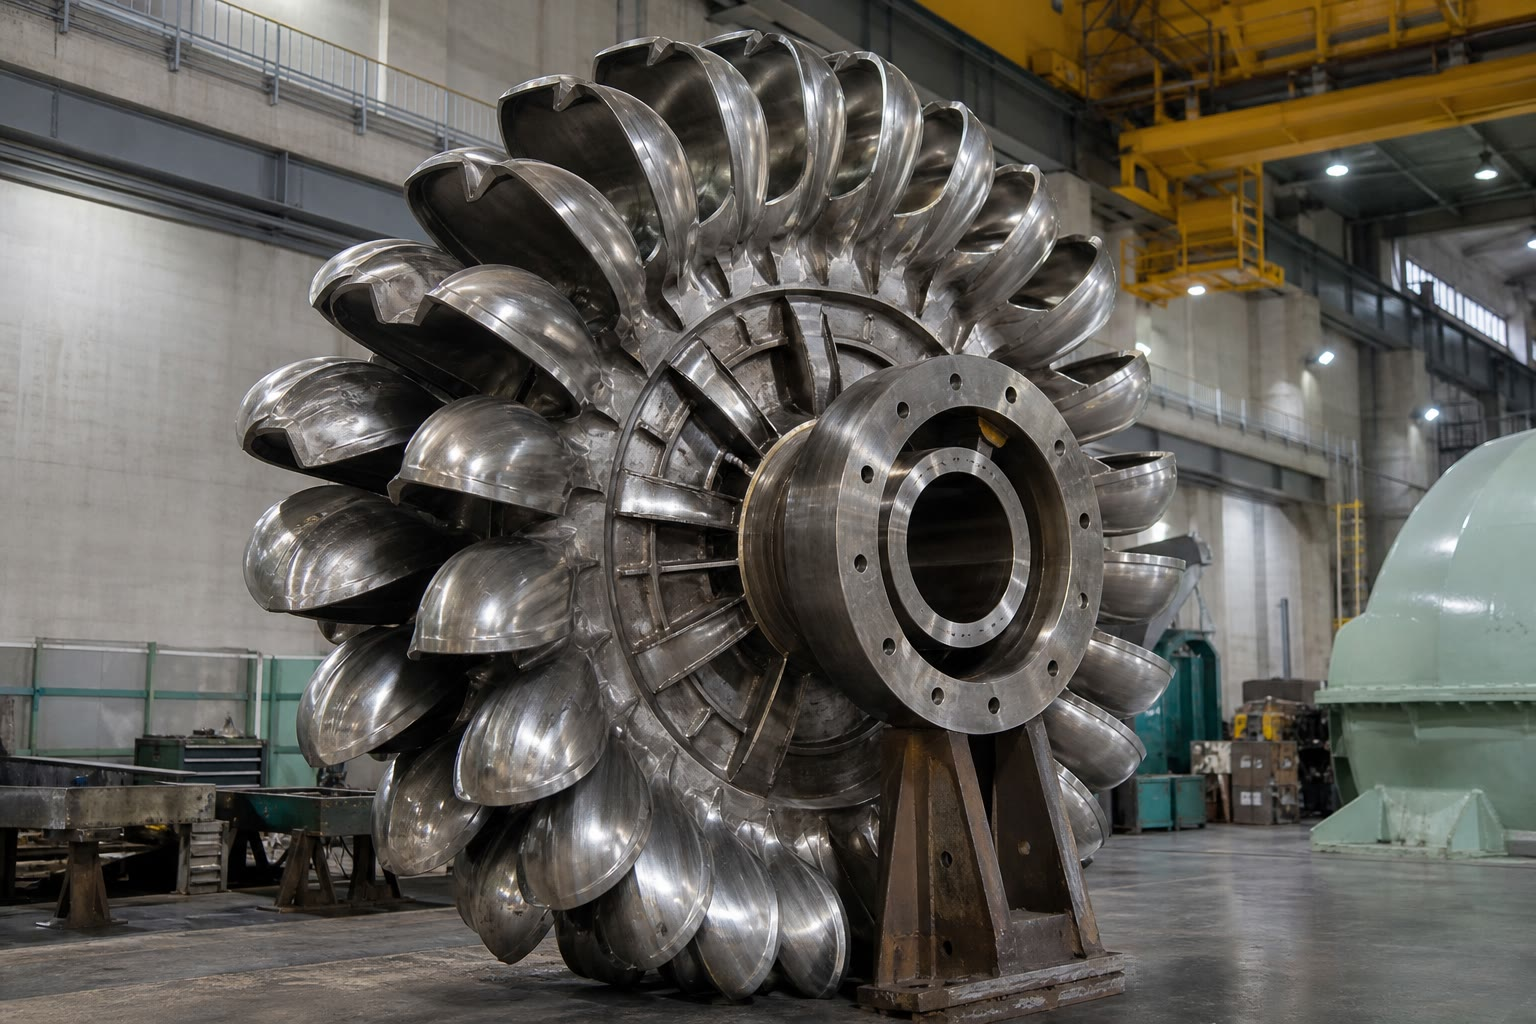
\includegraphics[width=0.58\linewidth]{images/book4/ai/b4-05-pelton-wheel.jpg}

{\small 佩尔顿水轮机的转轮：每个斗叶将射流几乎折回 $180^\circ$，水的动量变化即为作用在转轮上的力。}
\end{omfigure}

\begin{omfigure}
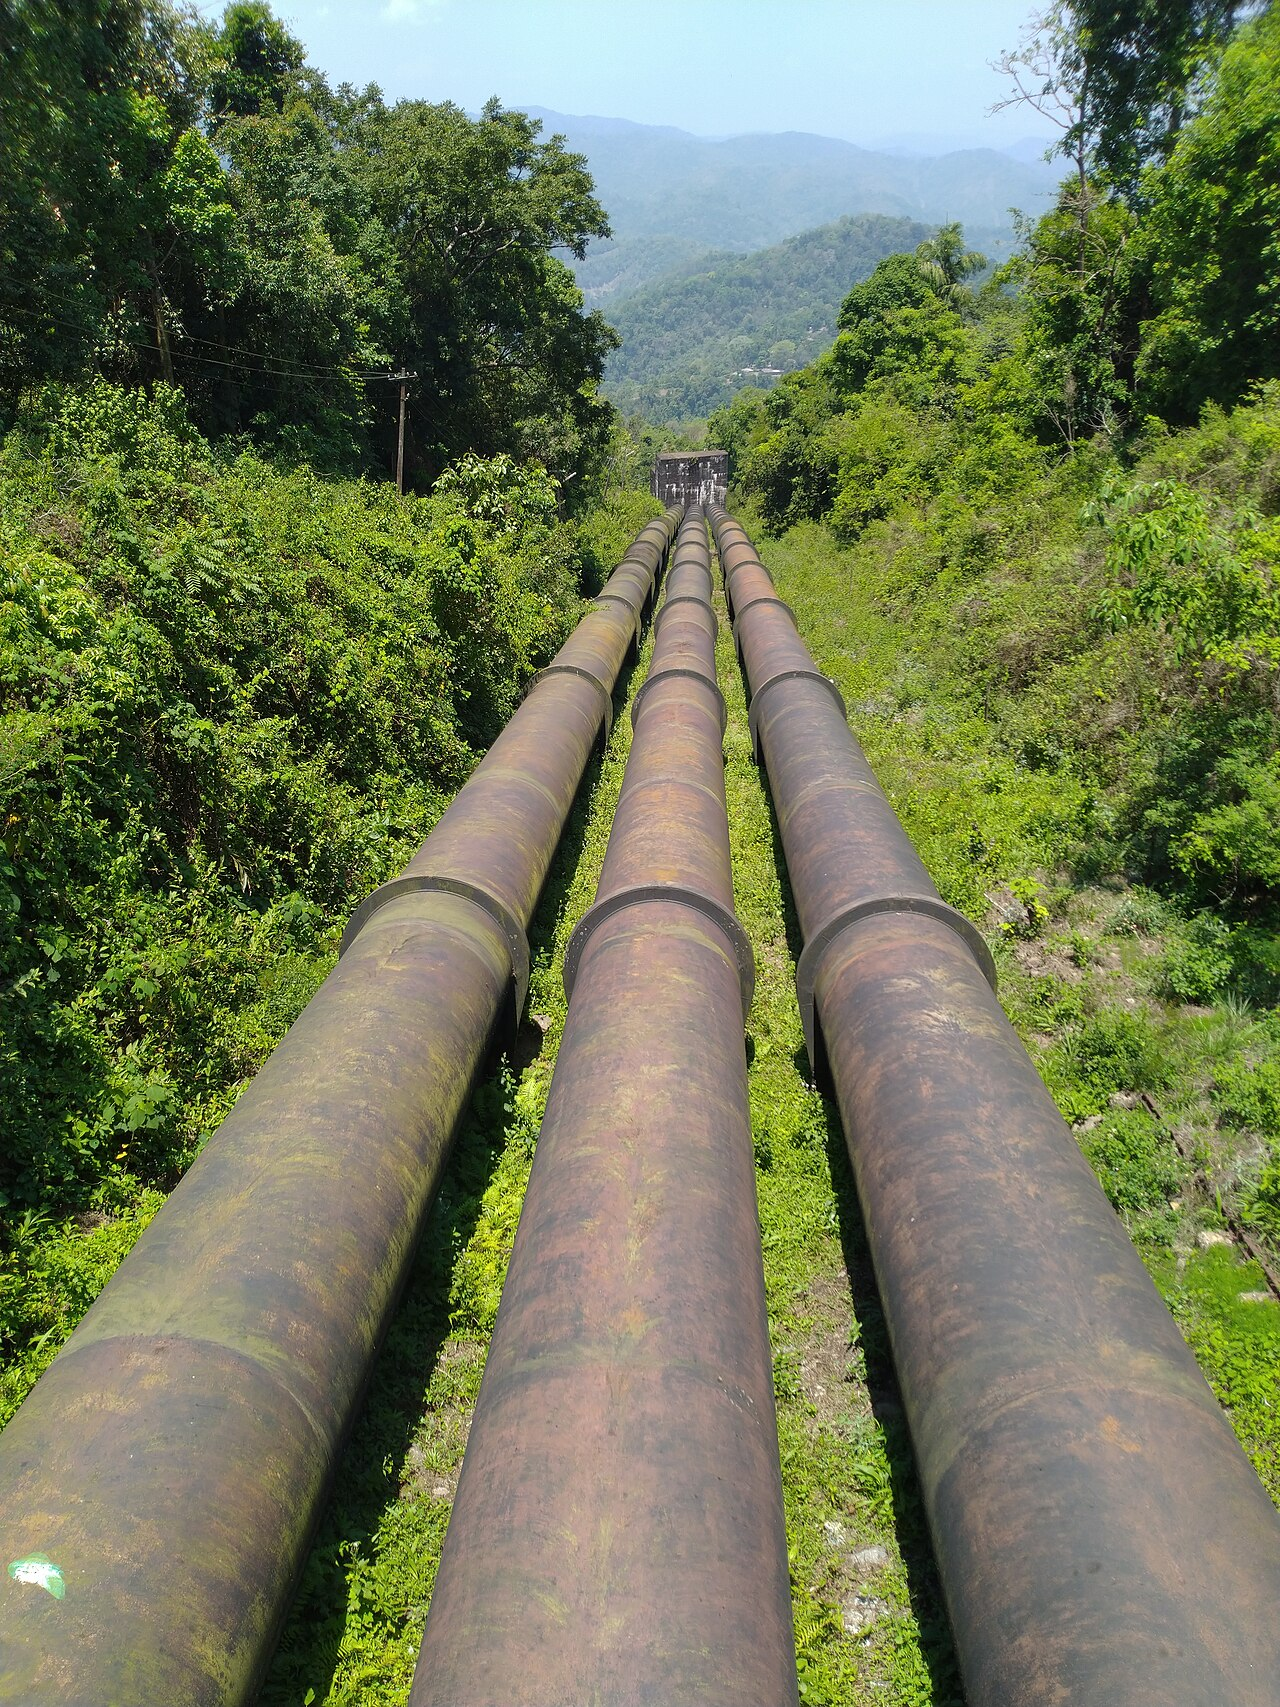
\includegraphics[width=0.42\linewidth]{images/book4/penstock-sabarigiri.jpg}

{\small 水电站的压力水管将水输送至下方的涡轮机：射流作用于佩尔顿水轮斗叶上的动量平衡，将水头转化为有用功。}
\end{omfigure}

\section{问题：射流、火箭与转轮}

\begin{problem}[{周末问题——什么推动喷气飞机，什么托起火箭，
什么驱动涡轮，
以及把水抽到高处要付出的代价}]
\label{pb:b2:flow-balances:1}

\medskip
\noindent\textbf{第一部分——涡轮喷气发动机。}
试验台上的一台发动机吸入 $D_a = \qty{50}{kg/s}$ 的静止空气，
燃烧 $D_f = \qty{1.0}{kg/s}$ 的燃料，并排出混合气体，其速度为 $v_e =
\qty{600}{m/s}$，压强为大气压强。
\begin{enumerate}
  \item 试验台上的推力。
  \item 飞行中速度为 $v = \qty{250}{m/s}$（相对发动机的排气速度仍为 $v_e$）时：
        推力，以及推进功率 $Fv$。
  \item 在发动机参考系中计算，传给气体的动能功率。
        推进效率 $\eta_p = Fv/\mathcal P_{\text{动}}$；
        证明：略去燃料质量时，$\eta_p = 2v/(v + v_e)$。
  \item 燃料的热值为 \qty{43}{MJ/kg}，求
        发动机的热效率（动能功率与热功率之比）及总效率。
  \item 涡扇发动机用相同的动能功率使
        $\qty{500}{kg/s}$ 的空气加速。求排气速度、推力及 $\eta_p$，在
        \qty{250}{m/s} 时的值。为什么民航客机要装巨大的风扇？
  \item 为什么涡轮喷气发动机不能承担火箭的任务，
        即在大气层之上工作？
  \item 着陆时的反推力使风扇气流向前偏转，
        与轴线成 \qty{45}{\degree}：求第 5 题中涡扇发动机的制动力，
        速度为 \qty{70}{m/s}，此时风扇排气相对发动机的速度为
        \qty{150}{m/s}；
        并与同一气流给出的向前推力作比较。
\end{enumerate}

\medskip
\noindent\textbf{第二部分——火箭。}
单级火箭：初始质量 $m_0 = \qty{300}{t}$，
其中推进剂质量为 \qty{200}{t}，排气速度 $v_e = \qty{3.0}{km/s}$，燃烧时间 $\tau =
\qty{150}{s}$，质量流量恒定。
\begin{enumerate}[resume]
  \item 对火箭加上 $\dd t$ 内喷出的气体，应用动量平衡，
        推导 $m\,\dd v/\dd t = D_mv_e - mg$，
        此式适用于竖直飞行。
  \item 质量流量、推力，以及起飞时与
        燃尽时的加速度。
  \item 积分求燃尽时的速度；何谓“重力
        损失”？
  \item 将同一火箭分为两级，每级各含 \qty{100}{t} 推进剂，求燃尽速度；
        第一级的空壳质量（\qty{20}{t}）在第二级点火前抛去
        （此处忽略重力），
        与单级情形作比较。
  \item 若要用相同的质量比使单级火箭达到轨道速度，
        （\qty{7.8}{km/s}，忽略重力），排气速度应为多少？
        请评述推进剂的选择。
  \item 起飞时，排气射流（质量流量 \qty{1333}{kg/s}、速度 \qty{3}{km/s}）
        撞击发射台的导焰板并被转为水平方向：
        求导焰板所受的力。
  \item 火箭的排气同样是流体流动：为什么对实际喷管而言，
        推力随海拔升高而\emph{增大}（可考虑喷口出口截面上的
        压强）？
\end{enumerate}

\medskip
\noindent\textbf{第三部分——佩尔顿水轮。}
上一章电站的射流：$D_V = \qty{60}{m^3/s}$，速度 $v =
\qty{62.6}{m/s}$，分配给两个水轮；每个水轮的半径 $R =
\qty{1.5}{m}$，斗叶使射流偏转 \qty{165}{\degree}。
\begin{enumerate}[resume]
  \item 斗叶速度为 $u$ 时一个水轮的斗叶所受的力，以及
        功率；求最优的 $u$。
  \item 最优情形下的转速（单位为 rpm）；轴上的力矩。
  \item 发电机的转速应为 \qty{50}{Hz} 的整数倍再除以
        其极对数；选取极对数。
  \item 单个水轮的功率，以及相对射流
        动能功率的效率；求发电机效率为 $95\%$ 时的
        总电功率。
  \item 对斗叶在最优情形下应用角动量平衡（欧拉涡轮方程）：
        进入与离开的水的角动量（每千克），
        并校核力矩。
  \item 负荷骤降，水轮向 $u =
        v$ 飞逸，作用力与力矩各如何变化，以及为何
        使射流偏离的导流器是每座佩尔顿电站的组成部分？
\end{enumerate}

\medskip
\noindent\textbf{第四部分——抽水至高处。}
电站还用作储能：夜间以 \qty{40}{m^3/s} 的流量
经压力水管（\qty{400}{m}、\qty{3}{m}、$\lambda = 0.015$）向上抽水，
抽至高出 \qty{200}{m} 的水库。
\begin{enumerate}[resume]
  \item 流量为 \qty{40}{m^3/s} 时压力水管中的水头损失，以及所需的泵扬程。
  \item 水力功率，以及泵效率为 $88\%$ 时的
        耗用的电功率。
  \item 抽水时压力水管底部的压强；
        与其在水轮机工况下的值（见上一章）作比较。
  \item 每夜 \qty{8}{h} 内储存的能量（被抬升水的
        势能）；储能的往返效率，设水轮机工况回收
        可用水头的 $90\%$，
        发电机效率为 $95\%$。
  \item 总结本题用到的四种平衡（动量、角动量、
        能量、质量），以及每一种平衡所设计的装置。
\end{enumerate}
\end{problem}
